% !TEX root = msc_thesis.tex

\chapter{Discussion} \label{ch:discussion}

The primary objective of this project was to extend ELASPIC and make it possible to predict the effect of mutations on protein stability and protein-protein interaction affinity on a genome-wide scale. We were able to meet this objective with a reasonable amount of success. We implemented ELASPIC as an easy to install and fully automated pipeline, which can scale from a single mutation in a user-provided PDB structure to hundreds of thousands of mutation affecting most proteins in the genome. ELASPIC can now be used as part of a pipeline for annotating variants discovered through high-throughput sequencing, since evaluating individual mutations takes minutes once the Provean supporting sets and homology models have been precalculated (see Section \ref{sec:precalculated_data}). With the work of Daniel Witvliet \textit{et al.} \cite{witvliet_elaspic_2016}, ELASPIC is also made accessible to the wider scientific community through a webserver.

The secondary objective of this project was to explore different approaches for using structural information in order to make more accurate and informative predictions regarding the phenotypic effect of mutations. We met the second objective with much less success than the first. Provean performs better than ELASPIC in predicting whether or not a mutation is involved in disease, as measured by the performance of the two tools on the validation and the test subsets of the Humsavar, ClinVar and COSMIC datasets (see Figures \ref{fig:core_validation} and \ref{fig:interface_validation}). While we found that mutations falling inside protein-protein interaction interfaces are more likely to be associated with disease, this may be an artifact of the fact that interfaces involved in disease are more likely to be studied to have a structural template of the interaction in the PDB. We found no evidence that ``edgetic mutations'' or mutations which affect only one of multiple interactions mediated by a protein, are more likely to be deleterious than mutations that destroy all interactions, as was reported by Sahni \textit{et al.} \cite{sahni_widespread_2015}.
% \cite{bordbar_personalized_2015} %
We could use ELASPIC in combination with kinetic models of cell metabolism or cell growth and replication \cite{karr_whole-cell_2012} in order to predict the effect of mutations on the corresponding phenotypes. However, even when used in combination with kinetic models of the cell, the $\Delta \Delta G$ predicted by ELASPIC may not be more informative than a deleteriousness score predicted by Provean or another sequence-based tool, particularly given the uncertainty that is associated with the predictions.

To our knowledge, this is the first study comparing the impact of mutations on protein stability and protein-protein interaction affinity with mutation deleteriousness on a genome-wide scale. At the outset of the project, we anticipated that analyzing the structural impact of mutations would allow us to predict not only whether or not a mutation is going to be deleterious but why it is going to be deleterious. One aspect of this study that we found promising was that mutation deleteriousness correlated well with the $\Delta \Delta G$ of core and interface mutations. This opens up the possibility of using mutation deleteriousness datasets to help train a more accurate $\Delta \Delta G$ predictor, instead of using $\Delta \Delta G$ predictions to try to decipher the link between mutations and disease. Two main factors limit the accuracy and the generalizability of ELASPIC. First, training datasets for both the core and interface predictors are limited in their accuracy and are biased in the types of mutations that they contain. This limitation could be addressed by allowing ELASPIC to be trained on mutations that affect multiple amino acids (see Section \ref{sec:more_data}). Second, most features that we calculate do not appear to be very informative, as shown in our feature elimination plots. The second limitation could be addressed by learning better mutations deleteriousness features, as described in section \ref{sec:better_features}.


\section{Adding support for multi-residue mutations} \label{sec:more_data}

One way to increase the amount of training data that is available for ELASPIC would be change ELASPIC to make it use experimental information for multi-residue mutations. ELASPIC can easily be extended to calculate the $\Delta \Delta G$ for mutations involving multiple amino acids. The tricky part is that the number of features changes with the number of amino acids that are mutated. We could address this by treating a mutation affecting multiple amino acids as a set of single amino acid mutations. For example, we could use the following recursive strategy:

% \vspace{-\topsep}
\begin{itemize}
	\itemsep0em
    \item Introduce each of the single amino acid mutations, one at a time.
    \item Select the single amino acid mutation with the most stabilizing effect.
    \item Repeat for the remaining mutations, using the structure containing the mutation selected in Step 2.
\end{itemize}

About one third on mutations in the Protherm and Skempi databases affect multiple amino acids. We could include those mutations in the training set by dividing them into single amino acid mutations and assigning to them a $\Delta \Delta G$ proportional to their contribution to the overall mutation score, as determined by the multiple amino acid substitution version of ELASPIC. This would require ``bootstrapping'' the ELASPIC predictor using single amin acid mutations, using the ``bootstrapped'' predictor to approximate the contribution of single amino acid mutaitons to the $\Delta \Delta G$ affecting mulitple amino acids, adding those mutations to the training set, and repeating.

In the case of the ELASPIC core predictor, we could create a dataset of multiple amino acid polymorphisms (MAAMs) from a thermophilic bacterium and it's closest non-thermophilic relative (maybe such a database already exists?). Cross-validate ELASPIC making sure that we predict those MAAMs to be stabilizing. Incorporate those MAAMs into our training set, weighting them accordingly.

In the case of the ELASPIC interface predictor, we could construct a dataset from phage-display read counts, and cross-validate ELASPIC while keeping track of its performance on phage display counts. Could then recursively incorporate the phage display data into the training set, weighting it by how well the ELASPIC predictor does on those mutations, as determined through cross-validation.

It is likely that the performance of the ELASPIC predictor would be lower for mutations affecting multiple amino acids than for mutations affecting a single amino acids, as the former is more likely to induce changes in the conformation of the protein that are not modelled by ELASPIC. This drop in performance could in-part be ameliorated by including a backbone relaxation step between each mutation, using molecular dynamics \cite{abraham_gromacs:_2015}, Rosetta Backrub \cite{smith_predicting_2011}, or other algorithms \cite{sun_protein_2016}.

If the ELASPIC predictor can achieve reasonable results for mutations affecting multiple amino acids, it could be used ``in reverse'' to design protein domains with increased stability and protein interfaces with increased affinity.



\section{Multitask learning of mutation deleteriousness and energetic effects} \label{sec:better_features}

In this work, we attempted to improve the generalizability of ELASPIC core and interface predictors by keeping track of their performance on mutation deleteriousness datasets throughout cross-validation and feature elimination (Figures \ref{fig:gridsearch_core}, \ref{fig:gridsearch_interface}, \ref{fig:feature_elimination_core} and \ref{fig:feature_elimination_interface}). While this approach allows us to discard predictors that overfit the training set, it does not improve the accuracy of any individual predictor.

One way to improve overall accuracy of the predictors would be to leverage information contained in mutation deleteriousness datasets to discover better and more useful features. Mutation deleteriousness datasets are much larger than the $\Delta \Delta G$ datasets, and they may allow sequential and structural features to ``mix'' in a more general environment, and produce combined features that are less noisy and better correlated with the actual effect of mutations.

We could learn those features by first training a boosted decision tree algorithm to predict mutation deleteriousness, and then use the output of those trees as input to a logistic regression model trained to predict mutation $\Delta \Delta G$ (Figure \ref{fig:multitask_learning}). The resulting predictor should not only have better accuracy, but also have a better ability to extrapolate than the currently-used gradient boosted regressor algorithm, which never predicts values that are higher or lower than the maximum or minimum value observed in the training set.

\begin{figure}[tb]
	\centering
	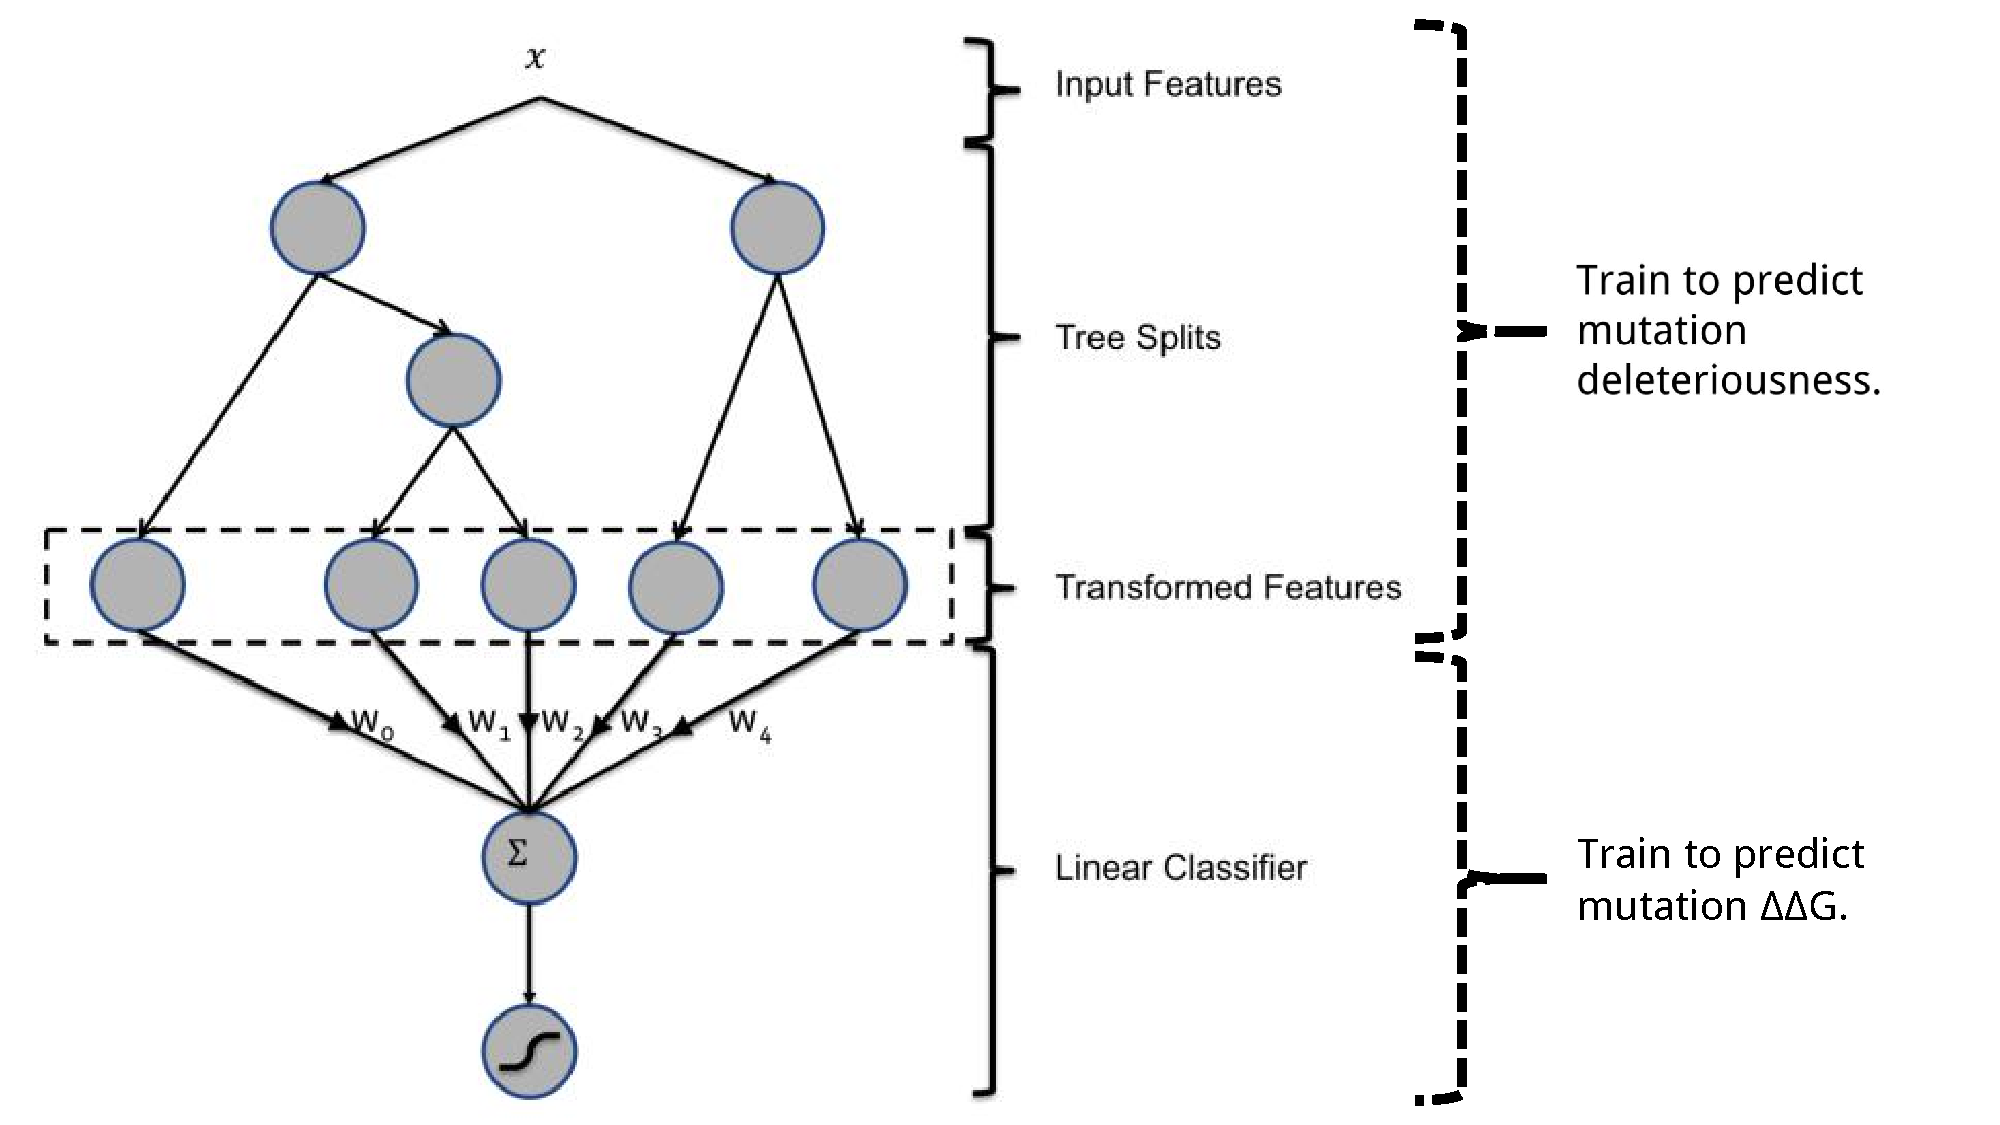
\includegraphics[width=0.8\textwidth]{static/elaspic/multitask_learning.pdf}
	\caption[Multitask learning of mutation deleteriousness and $\Delta \Delta G$.]{
		Multitask learning of mutation deleteriousness and $\Delta \Delta G$.
        The figure is adapted from He \textit{et al.} \cite{he_practical_2014}, where it is used to describe an algorithm that couples boosted decision trees and linear regression to predict add click-trough rate. Boosted decision trees are used to learn a feature ``manifold'' that is provided as input to the linear classifier, which in turn makes the final predictions. \\
        We propose to use a similar design, but train boosted decision trees to predict mutation deleteriousness, and fit a linear regressor to predict mutation $\Delta \Delta G$. We anticipate that the large training set of benign and deleterious mutations would allow the boosted decision tree algorithm to learn useful and generalizable features.
	}
	\label{fig:multitask_learning}
\end{figure}
